%! Author = David Nabergoj
%! Date = 26/01/2021

% Preamble
\documentclass[11pt, twocolumn]{article}

% Packages
\usepackage{graphicx}
\usepackage{amsmath}
\usepackage{amsfonts}
\usepackage[htt]{hyphenat}
\usepackage[
    top=20mm,
    bottom=20mm,
    left=20mm,
    right=20mm
]{geometry}
\usepackage{hyperref}
\hypersetup{
    colorlinks=true,
    linkcolor=red,
    urlcolor=blue,
    citecolor=black
}
\urlstyle{same}

%\newenvironment{comment}
%    {
%    \begin{center}
%    \begin{tabular}{|p{0.9\hsize}|}
%    \hline\\
%    \begin{footnotesize}\textbf{Comment:}}
%    {
%    \end{footnotesize}
%    \\\\\hline
%    \end{tabular}
%    \end{center}
%    }

\newenvironment{disclaimer}
    {
    \begin{center}
    \begin{tabular}{|p{0.9\hsize}|}
    \hline\\
    \begin{footnotesize}\textbf{Disclaimer:}}
    {
    \end{footnotesize}
    \\\\\hline
    \end{tabular}
    \end{center}
    }

% Title, author
\title{Reproducibility report: Walsh-Hadamard Variational Inference for Bayesian Deep Learning}
\author{David Nabergoj\thanks{University of Ljubljana, david.nabergoj@student.uni-lj.si %\href{mailto:david.nabergoj@student.uni-lj.si}{david.nabergoj@student.uni-lj.si}}
}}

% Document
\begin{document}
    \maketitle


    \section{Introduction}\label{sec:introduction}
    In this report, we assess the reproducibility of the paper ``Walsh-Hadamard Variational Inference for Bayesian Deep Learning''~\cite{rossi2019walsh}.
    We review the key contributions of the paper in Section~\ref{sec:brief-review-of-the-paper}.
    We state the most important findings to be reproduced and describe our approach to reproduce them in Section~\ref{sec:reproducibility-goals}.
    We describe the implementation details in Section~\ref{sec:implementation-details} and compare our empirical results to those in the original paper in Section~\ref{sec:running-the-experiments}.
    Finally, we conclude the report with an overall reproducibility assessment and discuss the clarity of the paper in Section~\ref{sec:conclusion-and-discussion}.
    Throughout this report, we describe our assumptions regarding the authors' intentions and why there might be discrepancies between our results and the original ones.
    The implementation of the proposed method, experiments and other files related to this report are available at \url{https://github.com/davidnabergoj/WHVI}.

    \begin{disclaimer}
    the author of this reproducibility report was not an expert in the related fields at the time of writing.
    The major results of this report are based on multiple readings of the original paper and its supplementary material~\cite{rossi2019walsh}, re-runs of the described experiments, as well as reading some key referenced literature~\cite{le2014fastfood, blundell2015weight, fino1976unified, kingma2015variational}.
    At the time of this study, there was no available code for the original paper, so all methods were implemented according to the listed literature.
    \end{disclaimer}

    \section{Brief review of the paper}\label{sec:brief-review-of-the-paper}
    The authors propose Walsh-Hadamard Variational Inference (WHVI), where weight matrices in Bayesian neural networks are efficiently re-parameterized to allow for linear space complexity and log-linear time complexity when transforming an input vector with a WHVI layer.
    The key idea is that weight matrices can be efficiently sampled by
    \begin{align}
        \widetilde{\mathbf{W}} = \mathbf{S_1} \mathbf{H} \mathrm{diag}(\widetilde{\mathbf{g}}) \mathbf{H} \mathbf{S_2},\quad\widetilde{\mathbf{g}} \sim q(\mathbf{g}).
        \label{eqn:weight-sampling}
    \end{align}
    Here, $\widetilde{\mathbf{W}}$ is a $D \times D$ weight matrix sample, $\mathbf{S_1}$ and $\mathbf{S_2}$ are deterministic diagonal matrices whose entries need to be optimized, $\mathbf{H}$ is the Walsh-Hadamard matrix, and $\widetilde{\mathbf{g}}$ is a sample from the distribution $q$.
    The variational posterior distribution $q$ is a multivariate normal distribution with a diagonal covariance matrix, i.e.\ $q(\mathbf{g}) = \mathcal{N}(\mathbf{\mu}, \mathbf{\Sigma})$.

    This approach offers an advantage over other approaches like Mean field Gaussian variational inference, because it requires $O(D)$ instead of $O(D^2)$ parameters to represent weight matrices of size $D \times D$.
    Furthermore, the matrix-vector product $\mathbf{Hx}$ can be computed in $O(D \log D)$ time and $O(1)$ space using the in-place version of the Fast Walsh-Hadamard transform.
    The described approach supports matrices of size $D \times D$ where $D = 2^p$ for $p > 0$ in its most basic form, however it is extended to support matrices of arbitrary size by concatenating smaller square matrices.

    WHVI is applied to a toy example, several regression and classification data sets, and is also tested on image classification tasks using Bayesian convolutional neural networks.

    \section{Reproducibility goals}\label{sec:reproducibility-goals}
    Our main goal is to implement all required procedures for WHVI and run the described experiments.

    Firstly, we would like to see similar results for the toy univariate regression example in section 3.1, Figure 4 of the original report.
    This primarily means obtaining qualitatively similar uncertainty estimates.
    Next, we will focus on the regression and classification data sets, as listed in Table 3 of the original report.
    We wish to obtain similar WHVI test error and WHVI test MNLL (mean negative log-likelihood) estimates, both the mean and the standard deviation.
    If our results vary significantly from the original ones, we will attempt to tune hyperparameters and report on the necessary changes.
    We will test the method across different random seeds to empirically assess stability and convergence.

    Due to empirically long training times for Bayesian neural networks, complex convolutional neural network architectures and the large number of parameters ($\sim 2.3M$), we will not be considering image clasification experiments in this report.
    We also believe they are not crucial to assessing the quality of the proposed approach.
    This is because the linear layers (not involving convolution operations) are already evaluated using standard regression and classification data sets, whereas the authors report that using WHVI for convolutional filters does not yield interesting results due to the small number of parameters.

    We will attempt to reproduce the findings regarding WHVI inference time to a smaller degree, because the workstation used in the experiments of the original paper is significantly more powerful than the one we used in this reproduction study.

    \section{Implementation details}\label{sec:implementation-details}
    \subsection{Core classes}\label{subsec:core-classes}
    We implemented WHVI in PyTorch~\cite{pytorch}, because it is also used in the original paper.
    One of the most important parts is the \texttt{WHVISquarePow2Matrix} class, which contains the parameters: elements of $\mathbf{S_1}$, $\mathbf{S_2}$, and the posterior mean $\mu$.
    It does not explicitly include elements of the diagonal covariance matrix $\Sigma$, but instead stores a parameter vector $\rho$ with $D$ elements, which corresponds to $\Sigma$ via a softplus transformation: $\Sigma = \mathrm{diag}(\sigma_1, \dots, \sigma_D)$ where $\sigma_i = \ln(1 + \exp(\rho_i))$.

    The authors do not state how they represent $\Sigma$.
    We chose the softplus transformation, because it was used in the seminal work on variational inference in neural networks~\cite{blundell2015weight}.
    The advantage is that we can optimize $\rho_i$ across the real line and disregard positivity constraints in the gradient-based optimization, then ensure non-negativity via a simple transformation.
    We acknowledge that the referenced work uses softplus for individual elements of the weight matrix, whereas we use it for elements of vector $\mathbf{g}$, which is indirectly related to the weight matrix via Equation~\ref{eqn:weight-sampling}.

    To transform a batch of input vectors, a weight matrix is sampled from the posterior according to Equation~\ref{eqn:weight-sampling} and multiplied by the matrix of the batch. See Subsection~\ref{subsec:sampling-the-weight-matrix} for details.

    The \texttt{WHVIStackedMatrix} class represents matrices of arbitrary size.
    It identifies how many smaller matrices of type \texttt{WHVISquarePow2Matrix} need to be stacked together to allow for the desired matrix multiplication, as well as the necessary padding of the input vector (see Algorithm 1 in the original report).
    These smaller matrices are stored in a \texttt{ModuleList} container as an attribute of \texttt{WHVIStackedMatrix}. When transforming a batch of input vectors, we generate one sample for each small matrix and concatenate these samples into a large matrix. The inputs are padded as necessary.

    As a special case, we also implement the \texttt{WHVIColumnMatrix} class, which transforms a batch of input vectors with a single element into a batch of output vectors with many elements.
    It includes a smaller \texttt{WHVISquarePow2Matrix}, which is sampled at input transformation time and reshaped into a column.
    The last few elements of this column may be removed to accomodate for the desired output size.
    This method is recommended in the paper and indeed reduces the number of parameters from $O(D)$ to $O(\sqrt{D})$, while also reducing the single-vector transform time complexity from $O(D\log D)$ to $O(\sqrt{D}\log D)$.
    Note that by transposing the sampled matrix, this class can be used to map many inputs to a single output.

    Finally, we create a \texttt{WHVILinear} layer class, which automatically selects the appropriate matrix based on the desired input and output dimensionalities.
    This is analogous to the traditional \texttt{Linear} layer in PyTorch, but also includes the computation of KL divergence $D_\mathrm{KL}\left(q(\mathbf{g}|\mu, \Sigma)\, ||\, p(\mathbf{g})\right)$ from the prior $p$ to the variational posterior $q$.
    The KL divergence of a \texttt{WHVILinear} layer is the sum of KL divergence terms for all of its descendants of type \texttt{WHVIStackedMatrix}.

    \subsection{Fast Walsh-Hadamard transform}
    An important contribution of the paper is the use of Fast Walsh-Hadamard transform (FWHT)~\cite{fino1976unified}, which allows for log-linear vector transformation time.
    We implemented the transform in Python and C++, both implementations can be used on the CPU and the GPU.
    We also adapted and tested a CUDA kernel implementation, which is considerably faster than the Python and C++ implementations on the GPU, but achieves speeds that are similar to the CPU implementations for $D \approx 2^7$.
    This was also observed by the authors.

    \subsection{Priors and parameter initializations}
    According to the supplementary material for the original paper, we use a zero-mean prior with fully factorized covariance $\lambda \mathbf{I}$ for a particular layer, i.e. $\mathcal{N}(\mathbf{0}, \mathrm{diag}(\lambda, \dots, \lambda)$ for a chosen $\lambda > 0$.

    We believe that the original paper should describe the choices of prior variances in more detail.
    Currently, the supplement seems to suggest that a constant $\lambda = 10^{-5}$ was used in all layers of the deep Bayesian networks, but this is likely not the case.
    Good choices of $\lambda$ are essential at each layer separately.
    We have found that with such a small prior covariance, the predictions are typically just the mean.
    However, by reconsidering the statement in the supplement, we may interpret it as putting a low prior covariance on the last layer and possibly higher ones on the previous layers.
    This indeed substantially improves the results of the experiments.

    The authors did not describe the initialization of $\mathbf{S_1}$, $\mathbf{S_2}$, $\Sigma$.
    We draw initial elements of $\mathbf{S_1}$ and $\mathbf{S_2}$ i.i.d.\ from a standard normal distribution and initial elements of $\rho$ i.i.d. from Uniform$(-3, -2)$.

    \subsection{Sampling the weight matrix}\label{subsec:sampling-the-weight-matrix}
    We implemented two forward pass options.
    In the first, we sample the weight matrix directly according to Equation~\ref{eqn:weight-sampling}.
    In the second, we use the local re-parameterization trick to sample the matrix-vector product $\mathbf{W}\mathbf{x} \in \mathbb{R}^D$ according to Equations~\ref{eqn:lrt1} and~\ref{eqn:lrt2}.

    \begin{align}
        \mathbf{W}\mathbf{x} = \overline{\mathbf{W}}(\mathbf{\mu})\mathbf{x} + \overline{\mathbf{W}}(\mathbf{\Sigma}^{1/2}\mathbf{\epsilon})\mathbf{x}, \; \epsilon \sim \mathrm{N}(\mathbf{0}, \mathbf{I}_D)\label{eqn:lrt1},\\
        \overline{\mathbf{W}}(u) = \mathbf{S_1} \mathbf{H} \mathrm{diag}(\mathbf{u}) \mathbf{H} \mathbf{S_2}\label{eqn:lrt2}
    \end{align}

    We explicitly build the Walsh-Hadamard matrix $\mathbf{H}$ on the CPU when $D < 2^{11}$.
    Like the authors, we found this to be a good trade-off point.
    For $D \ge 2^{11}$, we use the FWHT on the CPU.
    We always use the FWHT on the GPU, as it is faster than matrix multiplication.
    This agrees with the findings from the original paper.

    \section{Running the experiments}\label{sec:running-the-experiments}
    % TODO describe the details of how the experiments were run

    \subsection{Toy example}\label{sec:toy-example}
    In this section, we consider the toy example from Section 3.1, Figure 4 in the original paper.
    The authors do not provide an explicit formula for the function.
    To replicate the experiment as closely as possible, we look at the plot and roughly observe some $(x, y)$ pairs -- extrema and in-between values.
    We then use polynomial interpolation with a Vandermonde matrix to obtain a similar-looking function.
    This function is visualized in Figure~\ref{fig:toy-function}.

    \begin{figure}
        \centering
        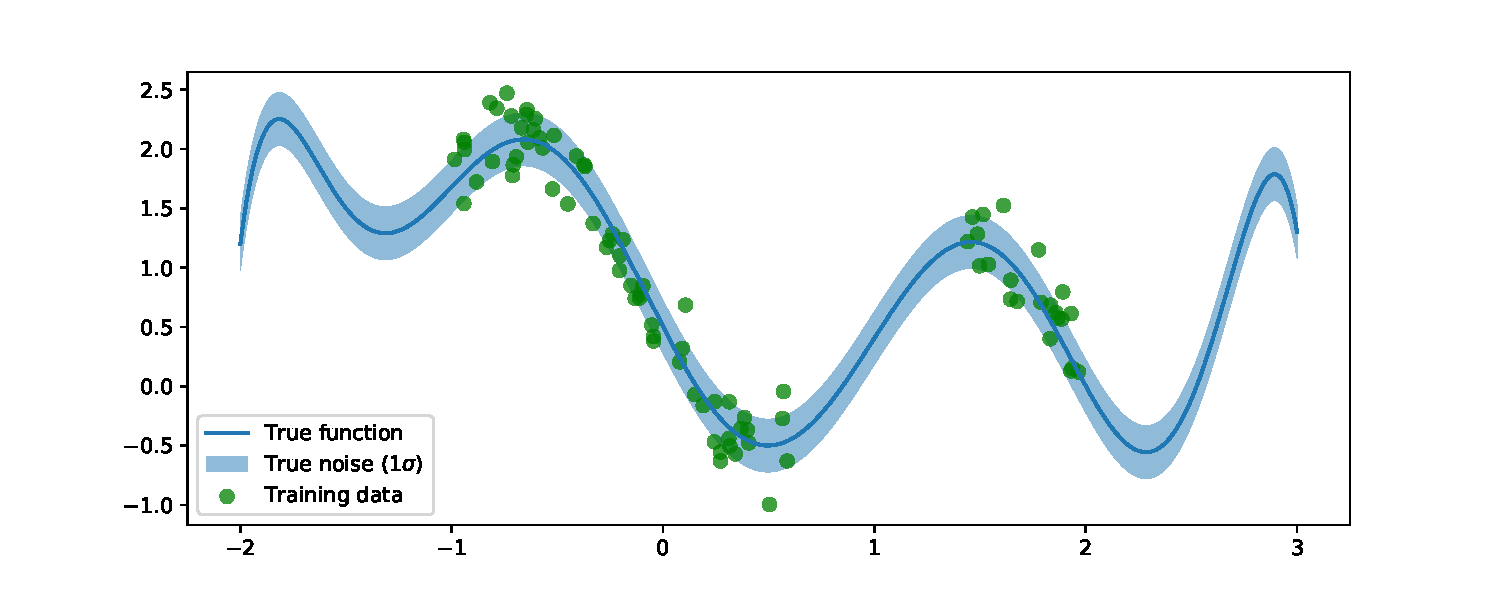
\includegraphics[width=1.0\hsize]{img/toy-function.pdf}
        \caption{Polynomial approximation to the toy function in the original paper.
        The exact form of this function up to two decimals is $f(x) = 0.50 -3.45x + 1.14x^2 + 4.36x^3 -0.93x^4 -1.77x^5 + 0.39x^6 + 0.22x^7 -0.06x^8$. The noise is normally distributed with $\sigma = \sqrt{\exp (-3)}$.
        }
        \label{fig:toy-function}
    \end{figure}

    The cosine activation function is no longer suitable given this different form of the function.
    We check this by training a non-Bayesian model, which has the exact same architecture as the WHVI one (two hidden layers with 128 hidden units).
    We found that the sigmoid activation performs slightly better and decided to use it in the WHVI experiment instead.
    A comparison of the two non-Bayesian models with different activations can be seen in Figure~\ref{fig:toy-function-non-bayesian}.

    \begin{figure}
        \centering
        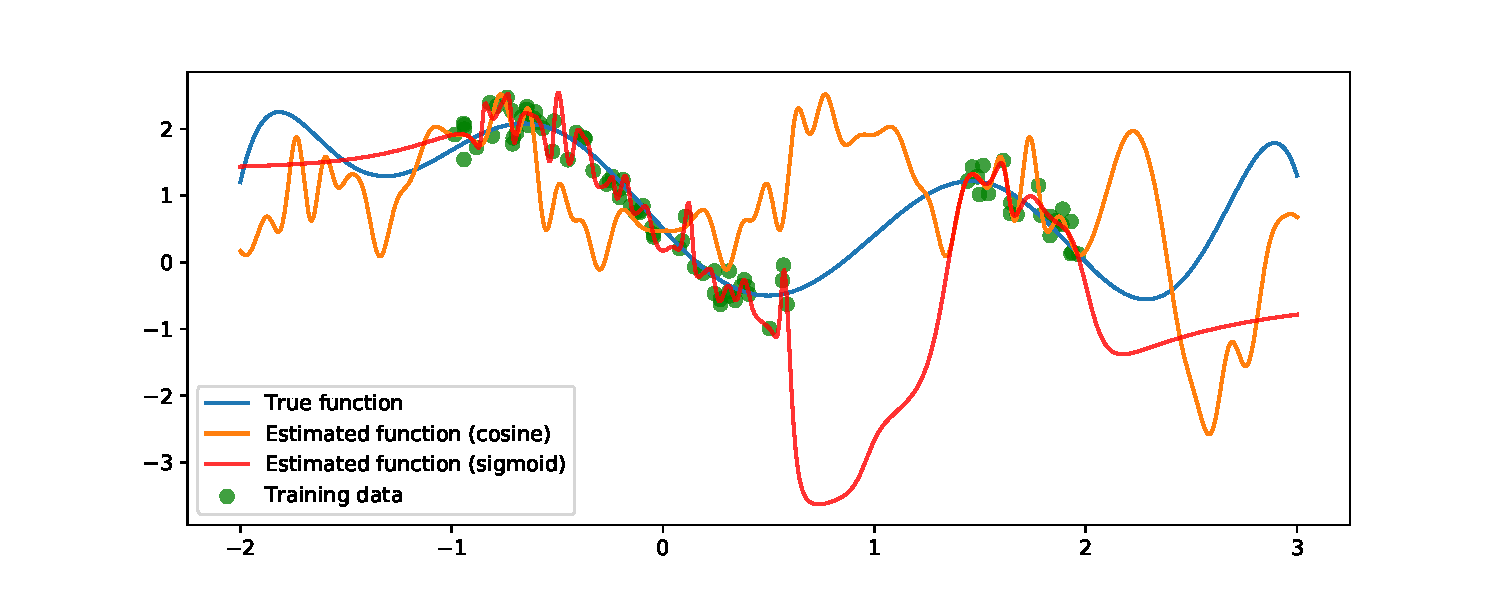
\includegraphics[width=1.0\hsize]{img/toy-function-non-bayesian.pdf}
        \caption{Comparison of the cosine and the sigmoid activation in a non-bayesian network.
        We decided to use sigmoid instead of cosine, because it seemed to capture the function more nicely on the left chunk of the data.}
        \label{fig:toy-function-non-bayesian}
    \end{figure}

    We trained the model with WHVI layers and found that the results depend heavily on initial $\lambda$ values in each layer as well as the initial scale $\sigma_0$ of the Gaussian likelihood.
    The result is visualized in Figure~\ref{fig:toy-function-whvi}.
    \begin{figure}
        \centering
        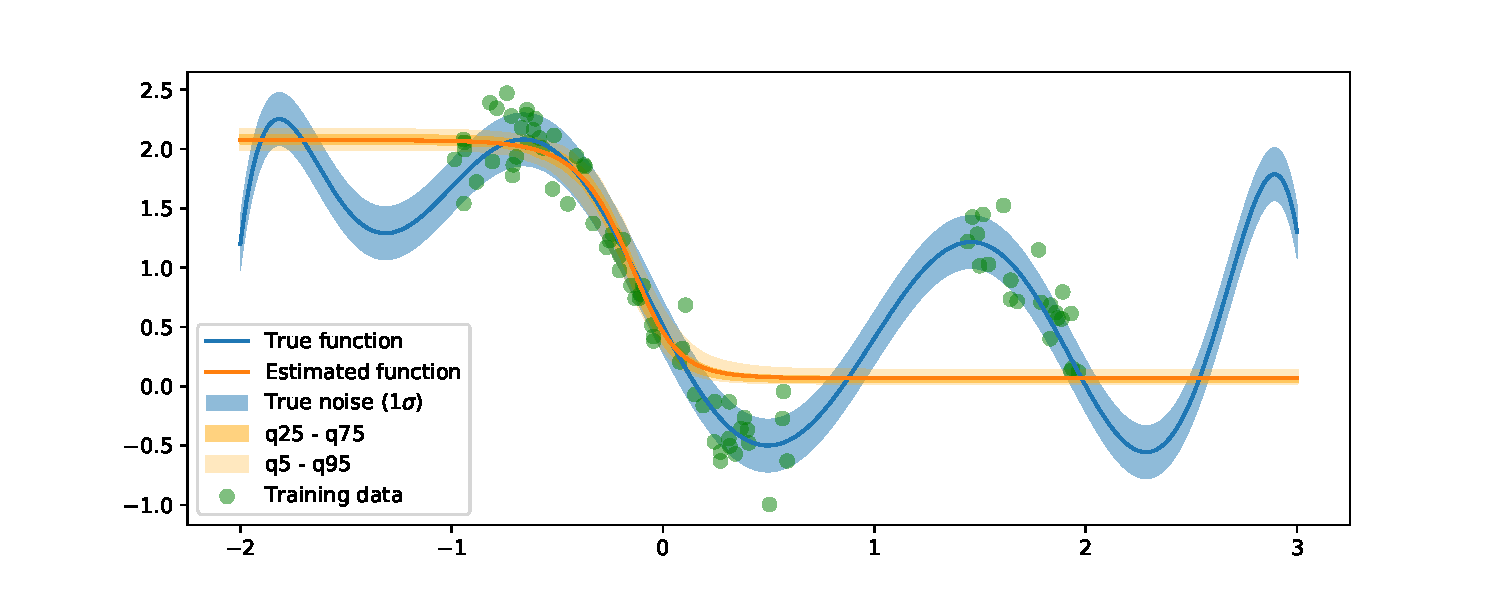
\includegraphics[width=1.0\hsize]{img/bayesian-fit-with-kl.pdf}
        \caption{
        Estimated function and the corresponding uncertainty.
        The dark-shaded region represents quantiles $q_{25}-q_{75}$, whereas the light-shaded one represents $q_{5}-q_{95}$.
        The underlying function is not modeled well.
        The model remains stuck in this local minimum even if we increase the number of epochs from 50000 to 200000.}
        \label{fig:toy-function-whvi}
    \end{figure}

    Many parameter choices resulted in slow convergence and significantly underestimated uncertainty.
    Our suggestions are to set $\lambda$ values that get gradually smaller as we approach the output layer and set $\sigma_0$ to be sufficiently larger than zero.
    In particular, our choices for modeling the toy data set were $\lambda_1=15, \lambda_2=5,\lambda_3=0.1, \sigma_0=5$.
    We also observed that the KL term in ELBO would often be much larger than the MNLL term at the beginning of the optimization. Conversely, the MNLL term would get stuck at suboptimal value and be unable to escape this local minimum even after several thousand epochs.
    After optimization, we observed several times that all but one pair of $\mu$ and $\Sigma$ parameters were almost exactly equal to zero and $\lambda$, indicating that the KL term was too dominant, drawing the variational posterior too close to the prior.

    The authors also state that they obtained a model with 1541 parameters for the toy example, however we obtained one with 1537 parameters.
    We were not able to identify the missing parameters and we believe that they are not hyperparameters, because the authors refer to hyperparameters separately in a Supplement section (i.e.\ not as ``parameters'').
    These missing parameters might be the solution to the observed problems in our experiments.
    As an experiment, we added bias columns (to be optimized) to WHVI layers to see if the performance would improve.
    This addition was not enough to obtain the desired results and also introduced a considerably large number of additional parameters.

    To conclude, we were not able to reproduce the uncertainty estimates, visualized in Figure 4 of the original paper.
    We suggest further research regarding parameter initialization.
    A possible solution would be to explore hyperpriors for $\mu$ and $\rho$ to allow for greater flexibility in the sampled weights.

    \subsection{Regression experiments}
    This section refers to experiments in section 3.2, Table 3 of the original paper.
    We use the experiment setup, described in section 3.2 of the original paper and section D.1 of the supplement.
    Again, the paper does not state the prior covariances $\lambda$ except for the last layer, where $\lambda = 10^{-5}$.
    We choose $\lambda = 3$ for all previous layers.

    The comparison between our results and the ones from the paper are presented in Table~\ref{tab:regression-experiments}.
    \begin{table*}[]
    \begin{tabular}{l|llll}
               & RMSE (original) & RMSE (ours) & { }MNLL (original) & MNLL (ours) \\ \hline
    Boston     & 3.14 (0.71)     &             & { }4.33 (1.80)     &             \\
    Concrete   & 4.70 (0.72)     &             & { }3.17 (0.37)     &             \\
    Energy     & 0.58 (0.07)     &             & { }2.00 (0.60)     &             \\
    KIN8NM     & 0.08 (0.00)     &             & -1.19 (0.04)       &             \\
    Naval      & 0.01 (0.00)     &             & -6.25 (0.01)       &             \\
    Powerplant & 4.00 (0.12)     &             & { }2.71 (0.03)     &             \\
    Protein    & 4.36 (0.11)     &             & { }2.79 (0.01)     &             \\
    Yacht      & 0.69 (0.16)     &             & { }1.80 (1.01)     &
    \end{tabular}
    \caption{WHVI regression experiments results. RMSE and MNLL are computed on test data sets. The result format is \textit{mean (std)}, where the sample mean and standard deviation are computed across 8 independent random train-test splits of the data sets.}
    \label{tab:regression-experiments}
    \end{table*}
    We were unable to reproduce the results, shown in the original paper.
    We believe that this is due to the missing parameters (see~\ref{sec:toy-example}) and possibly due to different values of $\lambda$.
    It is also possible that the authors invested more time into hyperparameter tuning to achieve such results, however we were unable to do the same given the considerable time and computational resources required for the described experiments.

    \section{Conclusion and discussion}\label{sec:conclusion-and-discussion}
    % TODO conclude with key findings regarding the reproducibility, discuss own results and authors' results.

    \bibliographystyle{unsrt}
    \bibliography{bibliography}

\end{document}